\chapter{DORIS System Theoretical Implications}
\label{ch:doris-theory}

\section{Introduction}
\label{sec:doris-introduction}

\begin{figure}
\centering
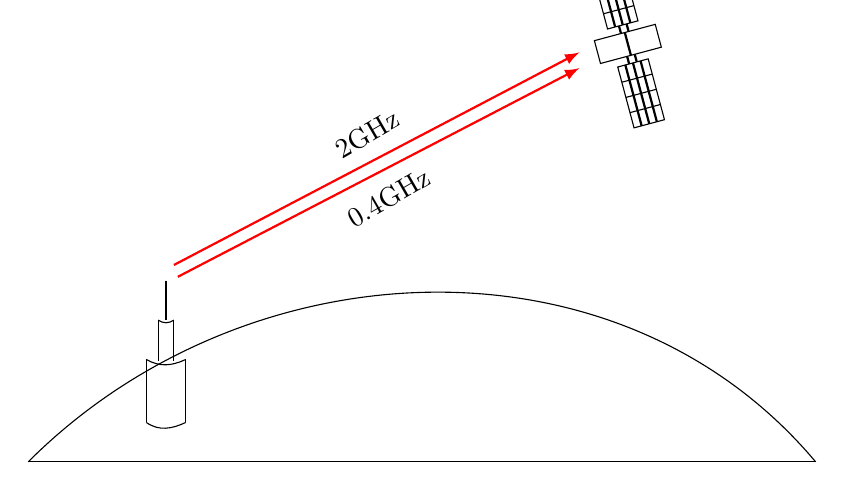
\begin{tikzpicture}
    \coordinate (lend) at (-5, 0);
    \coordinate (rend) at (5, 0);
    \draw (lend) to (rend);
    \draw (lend) to[out=45,in=-230] (rend);

    \coordinate (blb) at (-3.5, 0.5);
    \coordinate (brb) at (-3, 0.5);
    \draw (blb) to[out=-35,in=205] (brb);

    \coordinate (mlb) at (-3.5, 1.3);
    \coordinate (mrb) at (-3, 1.3);
    \draw (mlb) to[out=-30,in=205] (mrb);
    %\draw (mlb) to[out=35,in=-205] (mrb);
    \draw (blb) to (mlb);
    \draw (brb) to (mrb);
    
    \coordinate (tlb) at (-3.35, 1.8);
    \coordinate (trb) at (-3.15, 1.8);
    \draw (tlb) to[out=-35,in=215] (trb);
    \draw (tlb) to (-3.35, 1.28);
    \draw (trb) to (-3.15, 1.28);

    \coordinate (ulb) at (-3.26, 2.3);
    \coordinate (urb) at (-3.24, 2.3);
    \draw (ulb) to (-3.26, 1.8);
    \draw (urb) to (-3.24, 1.8);

    \rotatebox{15}{%
    \draw[] (3.5,4.6) rectangle (4.3,4.3);
    % Up panel
    \draw[thick] (3.9,4.3) to (3.9,4.6);
    \draw[thick] (3.85,4.6) to (3.85,4.7);
    \draw[thick] (3.95,4.6) to (3.95,4.7);
    \draw[] (3.7,5.5) rectangle (4.1,4.7);
    % grid
    \draw[thick] (3.8,4.7) to (3.8, 5.5); 
    \draw[thick] (3.9,4.7) to (3.9, 5.5); 
    \draw[thick] (4.0,4.7) to (4.0, 5.5); 
    \draw[] (3.7,4.9) to (4.1, 4.9);
    \draw[] (3.7,5.1) to (4.1, 5.1);
    \draw[] (3.7,5.3) to (4.1, 5.3);
    % Down panel
    \draw[thick] (3.85,4.3) to (3.85,4.2);
    \draw[thick] (3.95,4.3) to (3.95,4.2);
    \draw[] (3.7,3.4) rectangle (4.1,4.2);
    % grid
    \draw[thick] (3.8,3.4) to (3.8, 4.2); 
    \draw[thick] (3.9,3.4) to (3.9, 4.2); 
    \draw[thick] (4.0,3.4) to (4.0, 4.2); 
    \draw[] (3.7,3.6) to (4.1, 3.6);
    \draw[] (3.7,3.8) to (4.1, 3.8);
    \draw[] (3.7,4.0) to (4.1, 4.0);
    }
    
    \coordinate (satant1) at (2.0,  5.2);
    \coordinate (bcnant1) at (-3.15,2.5);
    \coordinate (satant2) at (2.0,  5.0);
    \coordinate (bcnant2) at (-3.10,2.35);
    \draw[thick,red,-latex] (bcnant1) -- node[above=1mm, align=center, black, rotate=30]{2GHz} (satant1);
    \draw[thick,red,-latex] (bcnant2) -- node[below=1mm, align=center, black, rotate=30]{0.4GHz} (satant2);

\end{tikzpicture}

\caption{DORIS System Description}
\label{fig:doris-system-description}
\end{figure}

\section{Theoretical Model of Doppler Observations}
According to \cite{lemoine-2016}, we define four basic events:
\begin{enumerate}
    \item beginning of emission of the 1\textsubscript{st} cycle by the emitter, 
    \(\tau_{e1}\) in the proper time scale of the emitter and \(t_1\) in the coordinate 
    time
    
    \item beginning of reception of the the 1\textsubscript{st} cycle by the receiver, 
    \(\tau_{r1'}\) in the proper time scale of the receiver and 
    \(t_{1'}\) in the coordinate time

    \item end of emission of the N\textsubscript{th} cycle by the emitter, 
    \(\tau_{e2}\) in the proper time scale of the emitter and \(t_2\) in the coordinate 
    time
    
    \item end of reception of the N\textsubscript{th} cycle by the receiver, 
    \(\tau_{r2'}\) in the proper time scale of the receiver and 
    \(t_{2'}\) in the coordinate time
\end{enumerate}

During the proper time interval \(\Delta\tau_{r} = \tau_{r2'} - \tau_{r1'}\), 
the receiver has received the \(N_e\) cycles sent by the emitter, with \(N_e = f_e \Delta\tau_e\), 
\(f_e\) being the proper frequency of the emitter. The receiver is also equipped with
an oscilator and during the proper time interval \(\Delta\tau_{r}\) has generated 
a number \(N_r = f_r \Delta\tau_r\) of cycles, \(f_r\) being the proper frequency of the 
receiver.

The Doppler measurement is the count, by the receiver electronics, of the number 
of cycles of difference between \(N_e\) and \(N_r\):
\begin{equation}
    \begin{split}
    N_{DOP} & = N_e - N_r\\
            & = f_e \Delta\tau_e - f_r \Delta\tau_r
    \end{split}
\end{equation}

\emph{In the RINEX files, this Doppler count is the difference between two phase measurements 
done at different time tags in the proper time-scale of the receiver.}

After a series of assumptions and simplifications, we can derive the theoretical 
formula for the Doppler count \cite{lemoine-2016}:
\begin{equation}
    \begin{split}
        \frac{c}{f_e \Delta\tau_r} N_{DOP} & \approx c \frac{f_e - f_r}{f_e} \\
        & - (1 - \frac{U_e}{c^2} - \frac{{V_e}^2}{2 c^2}) \frac{\rho_2 - \rho_1}{\Delta\tau_r}\\
        & + \frac{1}{c} (U_r - U_e + \frac{{V_r}^2 - {V_e}^2}{2}) \\
        & + \frac{2 \mu}{c^2 \Delta\tau_r} [\ln{(\frac{R_1 + R_{1'} + \rho_1}{R_1 + R_{1'} - \rho_1})} - \ln{(\frac{R_2 + R_{2'} + \rho_2}{R_2 + R_{2'} - \rho_2})}]
    \end{split}
\end{equation}

where \(U\) is the gravitational potential, \(V\) is the velocity of the clock, \(R\) 
is the geometric distance and \(\rho\) is the curvlinear trajectory (of the photon(s)).

The above equation can be (arbitrarily) split into two parts, one containing the ``measured'' 
quantities and one with the ``theoretical'' terms, as \cite{lemoine-2016}:
\begin{subequations}\label{eq:lem12}
  \begin{align}
    u_{measured} & = \frac{c}{f_e} (f_e - f_r -
     \frac{N_{DOP}}{\Delta\tau_r}) + \Delta u_{REL} \label{eq:lem12a} \\
    u_{theo}     &= \frac{\rho_2 - \rho_1}{\Delta\tau_r} (1- \frac{U_e}{c^2} - 
      \frac{{V_e}^2}{2 c^2}) \label{eq:lem12b}
  \end{align}
\end{subequations}

with
\begin{equation}
    \begin{split}
        \Delta u_{REL} &= \frac{1}{c} (U_r - U_e + \frac{{V_r}^2 - {V_e}^2}{2}) \\
        & + \frac{2 \mu}{c^2 \Delta\tau_r} [\ln{(\frac{R_1 + R_{1'} + \rho_1}{R_1 + R_{1'} - \rho_1})} - \ln{(\frac{R_2 + R_{2'} + \rho_2}{R_2 + R_{2'} - \rho_2})}]
    \end{split}
\end{equation}

We now need to introduce some additional corrections:
\(\Delta u_{IONO}\) and \(\Delta u_{TROPO}\), are the propagation corrections of 
the radio electric signal through the ionosphere and troposphere respectively. 

Additionaly, in the actual case (measurements), the nominal frequencies \(f_e\) and \(f_r\) 
are not the ``true'' ones; we hence need to apply a relative correction (e.g. for the 
emmiter) \(f_{e_T} = f_{e_N} (1 + \frac{\Delta f_e}{f_{e_N}})\), where the subscript \(T\) 
denotes the ``True'' frequency and \(N\) the nominal one. Thus in \ref{eq:lem12} the 
terms \(f_e\) and \(f_r\) need to be substituted by \(f_{e_T}\) and \(f_{r_T}\) respectively.

We will place \(\Delta u_{IONO}\) and \(\Delta u_{REL}\) (which do not involve adjusted parameters) 
on the ``measured'' part of \ref{eq:lem12} and \(\Delta u_{TROPO}\) and \(\frac{\Delta f_e}{f_{e_N}}\) 
on the ``theoretical'' part; neglecting some minor terms, we reach the equation \cite{lemoine-2016}:
\begin{subequations} \label{eq:lem13}
    \begin{align}
        u_{measured} & = \frac{c}{f_{e_N}} (f_{e_N} - f_{r_T} -
          \frac{N_{DOP}}{\Delta\tau_r}) + \Delta u_{REL} + 
          \Delta u_{IONO} \label{eq:lem13a} \\
        u_{theo} &= \frac{\rho_2 - \rho_1}{\Delta\tau_r} 
          (1- \frac{U_e}{c^2} - \frac{{V_e}^2}{2 c^2}) + 
          \Delta u_{TROPO} - \frac{c(\frac{N_{DOP}}{\Delta\tau_r} + 
          f_{r_T})}{f_{e_N}} \frac{\Delta f_e}{f_{e_N}} \label{eq:lem13b}
    \end{align}
\end{subequations}

where 
\begin{itemize}
    \item \(u_{measured}\) is the measured relative velocity between the emitter and 
    the receiver between the events 1' and 2', based on the Doppler count \(N_{DOP}\), 
    corrected for the ionospheric and relativistic effects.

    \item \(u_{theo}\) is the the theoretical (computed) emitter/receiver relative velocity 
    between the events 1' and 2', corrected for the tropospheric effect and for a solved-for 
    frequency bias \(\frac{\Delta f_e}{f_{e_N}}\) of the emitter. \(f_{r_T} = f_{r_N} (1 + \frac{\Delta f_r}{f_{r_N}})\) 
    is an estimate of the proper frequency of the receiver.

    \item \(\Delta u_{REL} = \Delta u_{{REL}_c} + \Delta u_{{REL}_r}\) is the relativistic 
    correction, composed of two parts: the clock correction \(\Delta u_{{REL}_c}\) and the 
    travel correction \(\Delta u_{{REL}_r}\)
    \begin{subequations} \label{eq:lem14}
        \begin{align}
            \Delta u_{{REL}_c} & = \frac{1}{c} 
              (U_r - U_e + \frac{{V_r}^2 - {V_e}^2}{2}) \label{eq:lem14a}\\
            \Delta u_{{REL}_r} & = \frac{2 \mu}{c^2 \Delta\tau_r} \left[ 
              \ln{(\frac{R_1 + R_{1'} + \rho_1}{R_1 + R_{1'} - \rho_1})} - 
              \ln{(\frac{R_2 + R_{2'} + \rho_2}{R_2 + R_{2'} - \rho_2})} \right] \label{eq:lem14b}
        \end{align}
    \end{subequations}
\end{itemize}

Note that \ref{eq:lem13} can be further simplified to \ref{eq:lem17} by 
ommiting small terms (\ref{ssec:small-terms}).

\emph{Usually, one frequency offset and one tropospheric zenithal bias are adjusted per pass.}

\section{Implementation of the Doppler Observation Model}

\subsection{Small Terms}
\label{ssec:small-terms}

In \ref{eq:lem13}, the smallest terms are \(-U_e / c^2 - {V_e}^2 / 2 c^2\) and 
\(\Delta u_{{REL}_T}\); in the case of DORIS they ammount to \num{11.} and 
\num{6.} \SI{10e-6}{\meter\per\second} respectively (\cite{lemoine-2016}). 
Furthermore, since the emitters are located on the ground, the term 
\(-U_e / c^2 - {V_e}^2 / 2 c^2\) is constant per station. This small 
relativistic offset is absorbed by the adjustment of \(\Delta f_e / f_{eN}\). 
So it is possibly to furher simplify \ref{eq:lem13} to:
\begin{subequations} \label{eq:lem17}
    \begin{align}
        u_{measured} & = \frac{c}{f_{e_N}} (f_{e_N} - f_{r_T} -
          \frac{N_{DOP}}{\Delta\tau_r}) + 
          \Delta u_{{REL}_C} + \Delta u_{IONO} \label{eq:lem17a}\\
        u_{theo} &= \frac{\rho_2 - \rho_1}{\Delta\tau_r} + \Delta u_{TROPO} - 
          \frac{c(\frac{N_{DOP}}{\Delta\tau_r} + f_{r_T})}{f_{e_N}} 
          \frac{\Delta f_e}{f_{e_N}} \label{eq:lem17b}
    \end{align}
\end{subequations}

\subsection{Correction of Aberration}

\subsection{Geopotential}
For a station on the geoid, the potential at the level of the station is the sum 
of the gravitational potential and the centrifugal potential due to the Earth's 
rotation: \(U_{GEO} = U_e + \frac{{V_e}^2}{2}\), which is a constant. For a station 
not located on the geoid, the quantity \(U_e + \frac{{V_e}^2}{2}\) will only depend 
on the height of the beacon above the geoid.

For the computation of the gravitational potential for \gls{leo} satellites, 
the pottential \(U_r\) cannot be restricted to the central term only and we must 
take into account the \(J_2\) term (at least, in addition to \(\mu / r\). The formula 
for the computation of the potential in this case is \cite{lemoine-2016}:
\begin{equation}
  \label{eq:lem18}
  U_r = \frac{\mu}{r} \left( 1- \left(\frac{\alpha_\Earth}{r}\right)^2 
    J_2 \frac{3 sin^2(\phi) - 1}{2} \right)
\end{equation}
with \(\alpha_\Earth\) the equatorial radious of the earth, \(r\) radial 
distance of the satellite (to the Earth's center), \(\phi\) latitude of the 
satellite and \(J_2 = 1.0826359 \dot 10^{-3}\) in the zero-tide system.

\subsection{True Proper Frequency of the Receiver}
\label{ssec:true-proprtfrequency-of-the-receiver}

For the term \(f_{r_T}\) that appears in \ref{eq:lem13}, we need an estimate of \(\Delta f_{r} / f_{r_N}\). 
This estimate can be obtained in one of the following ways \cite{lemoine-2016}:
\begin{enumerate}
    \item via the field ``F'' recorded for every single measurement in the DORIS 
    RINEX file (see \ref{ssec:relative-frequency-offset}); not that this estimation 
    is not very smooth, as noticed by \cite{GAO2015} and it is advisable, before 
    using it in \ref{eq:lem13}, to perform a linear (or polynomial) regression of 
    these estimates over one or a few days.

    \item It can also be obtained from a polynomial regression
    over the frequency offsets estimated during the passes
    over the master beacons

    \item It can finally be estimated by the users themselves as a
    by-product of their re-computation of the timetagging polynomial (see \cite{MERCIER2010})
\end{enumerate}

\subsection{Ionospheric Correction}
A first-order iono-free pseudo-range measurement on the \SI{2}{\GHz} channel is built by combining
the \SI{400}{\MHz} and \SI{2}{\GHz} measurements in the following way:
\begin{equation}
  C_{iono-free-2GHz} = \frac{\gamma C_{2GHz} - C_{400MHz}}{\gamma - 1}
\end{equation}
where \(\gamma\) is the square of the frequency ratio: 
\(\gamma = {(\frac{f_{2GHz}}{f_{400MHz}})}^2\).

Converting to iono-free phase measurement on the \SI{2}{\GHz} channel using 
\(c\)  the speed of light and \(L_{\alpha}\) is the phase measurements on the 
\(\alpha\) channel (\(\alpha\) = \SI{2}{\GHz} or \SI{400}{\MHz}), we get:

\begin{equation}
  \begin{aligned}
  L_{iono-free-2GHz} &= \frac{\gamma L_{2GHz} - 
    \sqrt{\gamma}L_{400MHz}}{\gamma - 1} \\
                     &= L_{2GHz} + \frac{L_{2GHz} - 
                        \sqrt{\gamma}L_{400MHz}}{\gamma - 1}
  \end{aligned}
\end{equation}

The coordinates of the iono-free phase centers are given by the following formula:
\begin{equation}
  \vec{\bm{r}}_{iono-free-2GHz} = \frac{\vec{\bm{r}}_{400MHz,2GHz}}{\gamma - 1}
\end{equation}
where \(\vec{\bm{r}}_{iono-free-2GHz}\) is the vector from the \SI{2}{\GHz} 
phase center to the iono-free phase center and \(\vec{\bm{r}}_{400MHz,2GHz}\) 
is the vector from the \SI{400}{\Hz} to the \SI{2}{\GHz} phase center. In 
DORIS, the iono-free phase centers are located a few mm away from the 
\SI{2}{\GHz} phase centers, in the direction opposite to the \SI{400}{\MHz} 
phase centers.
